\section{Análisis Dinámico del brazo}
Una vez resuelto el problema cinemático del brazo, se debe pasar a realizar un análisis dinámico del mismo. Comenzando por un análisis que nos muestre la relación que existe entre las intensidades aplicadas a los motores de las articulaciones del robot y las posiciones, velocidades y aceleraciones de dichas articulaciones.\\
Obteniendo así, un modelo dinámico del brazo manipulador; que nos permitirá desarrollar posteriormente todas las técnicas de control propuestas, por tanto, la fiabilidad, y la exactitud del modelo obtenido, determinaran en gran medida al control que se puedan desarrollar en este proyecto.


\subsection{Modelado Dinámico e Incertidumbres}
Como se ha comenzado diciendo, se ha de ser precavido en el desarrollo de este modelo dinámico, y mas aún, de cuanto podremos fiarnos de este.\\

En primer lugar, nos basamos en el modelo estructural que permite obtener dicha relación dinámica del motor de corriente continua:\\

	\begin{equation}
	K_tRI_m=(M(q)+J_mR^2)\ddot{q}+(C(q,\dot{q})+B_mR^2)\dot{q}+G(q)+F(\dot{q})
	\end{equation}\\

En la ecuación anterior, se tiene; en el término de la izquierda, las matrices de constantes de par de cada motor ($K_t$) y de reductoras ($R$) e intensidades ($I_m$) aplicadas a cada motor; por otro lado, en el término de la derecha encontramos las matrices de inercia de los eslabones ($M(q)$) y de los motores ($J_m$), la matriz de términos de Coriolis ($C(q,\dot{q})$) y la de términos viscosos de los motores ($B_m$), y las matrices de términos gravitatorios ($G(q)$) y de fricciones ($F(\dot{q})$), donde esta última no se tendrá en cuenta para la estimación del modelo.\\

Aparecen también los vectores columna $q$, $\dot{q}$ y $\ddot{q}$ que corresponden, respectivamente, a los valores de posición, velocidad y aceleración de las articulaciones.\\

Teniendo la ecuación matricial, se prosigue definiendo el contenido interno de estas matrices, donde entramos a considerar las incertidumbres dinámicas del robot. Estas son, en base a la estructura tomada:
\vspace{0.3cm}

\begin{itemize}
	\item Momentos de Inercia orden 0:
		\begin{center}
		$ m_0$ \hspace{0.2cm} $m_1$\hspace{0.2cm} $m_2$ \hspace{0.2cm}$m_3$
		\end{center}
	\item Momentos de Inercia orden 1:
		\begin{center}
		$ s_{11x}$\hspace{0.2cm} $s_{11y}$\hspace{0.2cm} $s_{11z}$\hspace{0.2cm}$ s_{22x}$\hspace{0.2cm}$ s_{22y}$\hspace{0.2cm}$ s_{22z}$\hspace{0.2cm}$ s_{33x}$\hspace{0.2cm}$ s_{33y}$\hspace{0.2cm}$ s_{33z} $
	\end{center}
	\item Momentos de Inercia orden 2:
		\begin{center}
		$ I_{11xx} $\hspace{0.2cm}$I_{11yy}$\hspace{0.2cm}$ I_{11zz}$\hspace{0.2cm}$ I_{22xx}$\hspace{0.2cm}$ I_{22yy}$\hspace{0.2cm}$ I_{22zz}$\hspace{0.2cm}$ I_{33xx}$\hspace{0.2cm}$ I_{33yy}$\hspace{0.2cm}$ I_{33zz} $
	\end{center}
	\item Inercia y Fricciones de Motores:
	\begin{center}
		$Jm_1$\hspace{0.2cm}$ Jm_2 $\hspace{0.2cm}$Jm_3$\hspace{0.2cm}$ Bm_1$\hspace{0.2cm}$ Bm_2$\hspace{0.2cm}$ Bm_3$
	\end{center}
\end{itemize}

\newpage

Tras definir las incógnitas inerciales, y el conocimiento geométrico del robot, se procede a la descripción interna de las
 matrices que definen nuestro modelo. Para ello, se va a realizar un método recursivo que se basa en la segunda ley de
 Newton denominado algoritmo de Newton-Euler, el cual obtiene los esfuerzos/pares aplicados en cada articulación.\\
 Dicho algoritmo ha sido proporcionado en clase por lo que no se explicará aquí; sí decir, que del robot sólo se conocen
 las longitudes de los eslabones y algunos parámetros dinámicos (reductoras y constantes de par) se realizará el cálculo
 con las incertidumbres dinámicas definidas como variables simbólicas que serán estimadas y sustituidas más adelante.\\

El resultado que se desea obtener con dicho algoritmo es el siguiente:\\
\begin{equation}
\tau=M(q)\ddot{q}+V(q,\dot{q})+G(q),
\end{equation}
donde el término $V(q,\dot{q})$ hace referencia al producto $C(q,\dot{q})\dot{q}$.\\

Como el algoritmo anterior obtiene el resultado total, se debe derivar el mismo para poder hallar las matrices aisladas. Por ello, el resultado $\tau$ se deriva respecto a $\ddot{q}$ para obtener la matriz $M(q)$. Acto seguido restar la matriz obtenida multiplicada por $\ddot{q}$ al valor de $\tau$ para eliminarlo y obtener las otras dos matrices.\\
\begin{equation}
M(q)=\dfrac{\partial{\tau}}{\partial{\ddot{q}}},
\end{equation}

El siguiente paso consiste en derivar la nueva $\tau$ respecto a la constante de gravedad $g$, puesto que aparece únicamente en los términos gravitatorios. Así, y multiplicando por $g$ a posteriori, se obtiene la matriz $G(q)$. Para hallar la matriz $V(q,\dot{q})$ basta con restar a la $\tau$ resultante de extraer la matriz de inercia la $G(q)$ anterior.\\
\begin{equation}
\tau_{new}=\tau-\dfrac{\partial{\tau}}{\partial{\ddot{q}}}\ddot{q},
\end{equation}

\begin{equation}
G(q)=\dfrac{\partial{\tau_{new}}}{\partial{g}},
\end{equation}

\begin{equation}
V(q,\dot{q})=\tau_{new}-G(q).
\end{equation}

Una de las características que hay que tener en cuenta del algoritmo de Newton-Euler es que no tiene en cuenta las viscosidades e inercias de los motores, por lo que hay que añadirlas a posteriori obteniendo las matrices $Ma(q)=M(q)+J_mR^2$ ; $Va(q,\dot{q})=V(q,\dot{q})+B_mR^2\dot{q}$ y $Ga(q)=G(q)$.\\

Una vez realizado todo esto se ha obtenido el modelo dinámico simbólico del robot, que se va a suponer correcto pues únicamente consiste en seguir unos pasos descritos en clase, pero que, si se desease, se podría comparar con un robot diseñado en Robotics Toolbox de Matlab asignando valores a los parámetros y realizando un mismo experimento para ambos modelos, tomando como referencia correcta el último de ellos.\\

Las ecuaciones dinámicas simbólicas que definen las articulaciones del robot se muestran a continuación: \\
\[
	\begin{pmatrix}
	\tau_{1} \\
	\tau_{2} \\
	\tau_{3}
	\end{pmatrix} =
	\begin{pmatrix}
		Ma_{1,1} & 0 & 0\\
		0 & Ma_{2,2} & Ma_{2,3}\\
		0 & Ma_{3,2} & Ma_{3,3}\\
	\end{pmatrix}
	\begin{pmatrix}
	\ddot{q_{1}} \\
	\ddot{q_{2}}  \\
	\ddot{q_{3}}
\end{pmatrix} +
\begin{pmatrix}
	Va_{1,1}\\
	Va_{2,1} \\
  Va_{3,1}
\end{pmatrix}
\begin{pmatrix}
		\dot{q_{1}} \\
		\dot{q_{2}}  \\
		\dot{q_{3}}
\end{pmatrix} +
\begin{pmatrix}
	0\\
	Ga_{2}\\
	Ga_{3}\\
\end{pmatrix}
\]

\newpage
A continuación se definirán las matrices que conforman las ecuaciones dinámicas del robot por separado: \\
La matriz asociada a los terminos inerciales del robot será:
\[
Ma=
\begin{bmatrix}
Ma_{1,1} & 0 & 0\\
0 & Ma_{2,2} & Ma_{2,3}\\
0 & Ma_{3,2} & Ma_{3,3}\\
\end{bmatrix} \]

\begin{itemize}
	\item $Ma_{1,1}= I_{11yy}+0.5I_{22xx}+0.5I_{22yy}+0.5I_{33xx} +0.5I_{33yy} - 0.5I_{22xx}cos(2q_{2})+0.5I_{22yy}cos(2q_2) +$ \\ \vspace{0.1cm}
	$+ Jm_1R_{1}^{2} + 0.5L_{2}^{2}m_{2} +0.5L_{2}^{2}m_{3}+ 0.5L_{3}^{2}m_{3}- 0.5I_{33xx}cos(2q_{2} + 2q_{3}) +0.5I_{33yy}cos(2q_{2} + 2q_{3}) +$ \\ \vspace{0.1cm}
	$+ m_{1}s{11z}^{2} + 0.5m_{2}s_{22x}^{2}+ 0.5m_{3}s_{33x}^{2}+ 0.5m_{2}s_{22x}^{2}cos(2q_{2})+ 0.5L_{3}^{2}m_{3}cos(2q_{2} + 2q_{3})+ $ \\ \vspace{0.1cm}
	$+ 0.5m_{3}s{33x}^{2}cos(2q_{2}+2q_{3}) - L_{2}m_{2}s_{22x}- L_{3}m_{3}s_{33x} + 0.5L_{2}^{2}m_{2}cos(2q_{2})+ 0.5L_{2}^{2}m_{3}cos(2q_{2})+ $ \\ \vspace{0.1cm}
	$+ L_{2}L_{3}m_{3}cos(q_{3}) -L_{2}m_{3}s_{33x}cos(q_{3})- L_{3}m_{3}s_{33x}cos(2q_{2} + 2q_{3})+L_{2}L_{3}m_{3}cos(2q_{2} + q_{3}) - $ \\ \vspace{0.1cm}
	$- L_{2}m_{3}s_{33x}cos(2q_{2} + q_{3})-L_{2}m_{2}s_{22x}cos(2q_{2})$ \\ \vspace{0.2cm}
	\item $Ma_{2,2}=I_{22zz}+I_{33zz}+Jm_{2}R_{2}^{2}+L_{2}^{2}m_{2}+L_{2}^{2}m_{3}+L_{3}^{2}m_{3}+m_{2}s_{s22x}^{2}++m_{3}s_{s33x}^{2}- 2L_{2}m_{2}s_{22x} - $ \\ \vspace{0.1cm}
	$ + 2L_{3}m_{3}s_{33x}+ 2L_{2}L_{3}m_{3}cos(q_{3}-2L_{2}m_{3}s_{33x}cos(q_{3})$ \\ \vspace{0.2cm}
	\item $Ma_{2,3}=m_{3}L_{3}^{2}- 2L_{3}m_{3}s_{33x}+L_{2}L_{3}m_{3}cos(q_{3})+m_{3}s_{33x}^{2}-L_{2}m_{3}s_{33x}cos(q_{3})+I_{33zz}$ \\ \vspace{0.2cm}
	\item $Ma_{3,2}=I_{33zz}+m_{3}(L_{3}-s_{33x})(L_{3}-s_{33x}+L_{2}cos(q_{3}))$ \\ \vspace{0.2cm}
	\item $Ma_{3,3}=I_{33zz}+Jm_{3}R_{3}^{2}+m_{3}(L_{3}-s_{33x})^{2}$ \\ \vspace{0.2cm}
\end{itemize}

La matriz asociada a los terminos de Coirolis del robot será:
\[
Va=
\begin{pmatrix}
Va_{1}\\
Va_{2}\\
Va_{3}\\
\end{pmatrix} \]
\begin{itemize}
	\item $Va_{1}=Bm_{1}\dot{q_{1}}R_{1}^{2} -\dot{q_{1}}(I_{33yy}\dot{q_{2}} sin(2q_{2}+2q_{3})) -I_{33xx}\dot{q_{3}} sin(2q_{2}+2q_{3}) +I_{33yy}\dot{q_{3}}sin(2q_{2}+2q_{3})- $ \\ \vspace{0.1cm}
	$ -I_{22xx}\dot{q_{2}} sin(2q_{2}) +I_{22yy}\dot{q_{2}} sin(2q_{2}) +  m_{3}\dot{q_{2}}s_{33x}^{2}sin(2q_{2}+2q_{3}) + m_{3}\dot{q_{3}}s_{33x}^{2}sin(2q_{2}+2q_{3}) +$ \\ \vspace{0.1cm}
  $  +L_{2}^{2}m_2 \dot{q_{2}}sin(2q_{2}) + L_{2}^{2}m_{3}\dot{q_{2}}sin( 2q_{2}) +  m_{2}\dot{q_{2}}s_{22x}^{2}sin(2q_{2}) +L_{3}^{2}m_{3} \dot{q_{2}}sin(2q_{2}+2q_{3}) +$ \\ \vspace{0.1cm}
	$ + L_{3}^{2}m_{3} \dot{q_{3}}sin(2q_{2}+2q_{3}) +  2L_{3}L_{2}m_{3} \dot{q_{2}}sin(2q_{2}+q_{3}) +L_{3}L_{2}m_{3} \dot{q_{3}}sin(2q_{2}+q_{3}) - $ \\ \vspace{0.1cm}
	$ -2L_{2}m_{3}\dot{q_{2}}s_{33x}sin(2q_{2}+q_{3})- L_{2}m_{3}\dot{q_{3}}s_{33x}sin(2q_{2}+q_{3}) -2L_{2}m_{2}\dot{q_{2}}s_{22x}sin(2q_{2}) +$ \\ \vspace{0.1cm}
	$ +L_{3}L_{2}m_{3} \dot{q_{3}}sin(q_{3}) -L_{2}m_{3} \dot{q_{3}}s_{33x}sin(q_{3}) -2L_{3}m_{3}\dot{q_{2}}s_{33x}^{2}sin(2q_{2}+2q_{3}) - 2L_{3}m_{3}\dot{q_{3}}s_{33x}^{2}sin(2q_{2}+2q_{3})  $ \\ \vspace{0.2cm}

	\item $Va_{2}=0.5I_{33yy}\dot{q_{1}}^{2}sin(2q_{2}+2q_{3}) -0.5I_{33xx}\dot{q_{1}}^{2}sin(2q_{2}+2q_{3}) +Bm_{2}R_{2}^{2}\dot{q_{2}} -0.5I_{22xx}\dot{q_{1}}^{2}sin(2q_{2})+ $ \\ \vspace{0.1cm}
	$+0.5I_{22yy}\dot{q_{1}}^{2}sin(2q_{2}) +0.5L_{3}^{2}m_{3} \dot{q_{1}}^{2}sin(2q_{2}+2q_{3}) +0.5m_{3}\dot{q_{1}}^{2}s_{33x}^{2}sin(2q_{2}+2q_{3}) $ \\ \vspace{0.1cm}
  $+0.5L_{2}^{2}m_{2} \dot{q_{1}}^{2}sin(2q_{2}) +0.5L_{2}^{2}m_{3} \dot{q_{1}}^{2}sin(2q_{2}) +0.5m_{2} \dot{q_{1}}^{2}s_{22x}^{2}sin(2q_{2}) $ \\ \vspace{0.1cm}
	$-L_{3}L_{2}m_{3} \dot{q_{3}}^{2}sin(q_{3}) +L_{2}m_{3}\dot{q_{3}}^{2}s_{33x}sin(q_{3}) -L_{3}m_{3}\dot{q_{1}}^{2}s_{33x}sin(2q_{2}+2q_{3}) $ \\ \vspace{0.1cm}
	$ +L_{3}L_{2}m_{3} \dot{q_{1}}^{2}sin(2q_{2}+q_{3}) -L_{2}m_{3}\dot{q_{1}}^{2}s_{33x}sin(2q_{2}+q_{3}) -L_{2}m_{2}\dot{q_{1}}^{2}s_{22x}sin(2q_{2}) $ \\ \vspace{0.1cm}
	$-2L_{3}L_{2}m_{3} \dot{q_{3}}\dot{q_{2}}sin(q_{3}) +2L_{2}m_{3} \dot{q_{2}}\dot{q_{3}}s_{33x}sin(q_{3}) $ \\ \vspace{0.2cm}

	\item $Va_{3}=0.5I_{33yy}\dot{q_{1}}^{2}sin(2q_{2}+2q_{3}) -0.5I_{33xx}\dot{q_{1}}^{2}sin(2q_{2}+2q_{3}) +Bm_{3}R_{3}^{2}\dot{q_{3}} $ \\ \vspace{0.1cm}
	$ +0.5L_{3}^{2}m_{3} \dot{q_{1}}^{2}sin(2q_{2}+2q_{3}) +0.5m_{3}\dot{q_{1}}^{2}s_{33x}^{2}sin(2q_{2}+2q_{3}) +0.5L_{3}L_{2}m_{3} \dot{q_{1}}^{2}sin(q_{3}) $ \\ \vspace{0.1cm}
	$+L_{3}L_{2}m_{3} \dot{q_{2}}^{2}sin(q_{3}) -0.5m_{3}L_{2}\dot{q_{1}}^{2}s_{33x}sin(q_{3}) -m_{3}L_{2}\dot{q_{2}}^{2}s_{33x}sin(q_{3}) $ \\ \vspace{0.1cm}
	$-L_{3}m_{3}\dot{q_{1}}^{2}s_{33x}sin(2q_{2}+2q_{3}) +0.5L_{2}L_{3}m_{3}\dot{q_{1}}^{2}sin(2q_{2}+q_{3}) -0.5L_{2}m_{3}\dot{q_{1}}^{2}s_{33x}sin(2q_{2}+q_{3})$ \\
\end{itemize}

La matriz asociada a los terminos gravitatorios del robot será:
	\[
	Ga=
	\begin{pmatrix}
	0\\
	Ga_{2}\\
	Ga_{3}\\
	\end{pmatrix} \]

	\begin{itemize}
		\item $Ga_{2}=g(L_{3}m_{3}cos(q_{2}+q_{3})-m_{2}s_{22x}cos(q_{2})-m_{3}s_{33x}cos(q_{2}+q_{3})+L_{2}m_{2}cos(q_{2})+L_{2}m_{3}cos(q_{2})) $ \\ \vspace{0.1cm}
		\item $Ga_{3}=g*m_{3}cos(q_{2}+q_{3})(L_{3}-s_{33x})$ \\
	\end{itemize}

	\subsection{Obtención de los parámetros dinámicos del robot}
	Al obtener las matrices del modelo dinámico, ya seremos capaces de predecir el comportamiento de nuestro robot en la realidad;
una vez que determinemos las incertidumbres paramétricas que se especificaron al inicio del apartado anterior.
Osea se, que aunque tengamos estructuradas las matrices, no seremos capaces de determinar el comportamiento
del robot, ya que, tenemos un compendio de incertidumbres, que deberán ser determinadas numéricamente.\\

Por tanto, este apartado esclarecerá como resolver las incertidumbres paramétricas presentes, mediante
técnicas de regresión lineal y la realización de experimentos sobre el propio robot, para determinar las siguientes
incógnitas definidas en Matlab como variables simbólicas:

	\subsubsection{Identificalion y Linealizacion de parámetros dinámicos}
		Primero reestructuraremos nuestro modelo dinámico en dos matrices en las que, por un lado,
		se agrupen las incertidumbres paramétricas en una matriz \textit{theta}, y por otro, el resto de nuestro modelo
		dinámico en una matriz \textit{phi} que dependerá de las variables articulares del robot.

		\begin{equation}
			\tau=M(q)\ddot{q}+V(q,\dot{q})+G(q) \hspace{1.25cm}  \rightarrow \hspace{1.25cm} \tau=\phi(x) \hspace{0.25cm} \theta
			\end{equation}


	Agrupando en \textit{theta} el conjunto de las incertidumbres obtenemos el vector de términos resultante.
	\begin{equation}
		\theta=
			\begin{pmatrix}
				I_{11xx} \\
				I_{11yy}\\
				I_{11zz}\\
				Jm_{1} \\
				Bm_{1} \\
				I_{22xx} \\
				I_{22yy}\\
				I_{22zz}\\
				Jm_{2} \\
				Bm_{2} \\
				I_{33xx} \\
				I_{33yy}\\
				I_{33zz}\\
				Jm_{3} \\
				Bm_{3} \\
				m_{1}s_{11z}^{2} \\
				m_{1}s_{11z} \\
				m_{1}\\
				m_{2}s_{22x}^{2} \\
				m_{2}s_{22x} \\
				m_{2}\\
				m_{3}s_{33x}^{2} \\
				m_{3}s_{33x} \\
				m_{3}
				\end{pmatrix}
		\end{equation}

		Si usamos este vector \textit{theta} como base para re-ordenar nuestro modelo dinámico, vemos, en la matriz resultante \textit{phi},
		que existen columnas repletas de ceros, o relaciones lineales entre las columnas, por lo que, se deberán
		agrupar aquellos términos que no sean linealmente independientes y eliminar los términos asociados
		a las columnas de ceros, ya que significará que no tienen relevancia en nuestro modelo dinámico.\\

		Para poder agrupar los parámetros linealmente independientes, nos apoyaremos en Matlab para poder gestionar
		estas matrices de gran tamaño.\\
		Se deben asignar valores aleatorios a los parámetros articulares que aparecerán en la matriz \textit{phi}, y sustituir estos
		valores dentro de la matriz; posteriormente se elegirán otros valores para las variables articulares,  y se concatenarán
		con la matriz anterior. Este proceso se repetirá hasta obtener una matriz concatenada de iguales dimensiones de ancho y largo.\\

		Obteniendo esta matriz cuadrada podremos ejecutar el comando \textit{rref()} que nos devolverá las relaciones entre las columnas de la matriz \textit{phi}, y que serán las mismas relaciones dentro de las filas del vector de incertidumbres \textit{theta}.\\

Por tanto, la matriz $\theta$ linealmente independiente obtenida será:
			\[
			\theta=
				\begin{pmatrix}
					  m_{1}s_{11z}^{2} + m_{2}s_{22x}^{2} + m_{3}s_{33x}^{2} + I_{11yy} + I_{22yy} + I{33yy} + R_{1}^{2}Jm_1 - m_2 - 1.64m_3 \\
					  Bm_{1}  \\
					  -m_{2}s_{22x}^{2} + I_{22xx} - I_{22yy} + m_{2} + m_{3} \\
					  m_{2}s_{22x}^{2} + I_{22zz} + R_{2}^{2}Jm_{2} - m_{2} - m_{3}  \\
					  Bm_{2} \\
					  - m_{3}s_{33x}^{2} + I_{33xx} - I_{33yy} + 0.64m_{3} \\
					  m_{3}s_{33x}^{2} + I_{33zz} - 0.64m_{3}  \\
					  Jm_{3}  \\
					  Bm_{3}  \\
					  -m_{2} -m_{3} + m_{2}s_{22x}  \\
					  m_{3}s_{33x} - 0.8m_{3}
				\end{pmatrix}
			\]

\vspace{1cm}
Por otro lado, la matriz $\gamma$ obtenida, la cuál únicamente también posee términos linealmente independientes, se muestra a continuación:
			\[
\gamma=
\begin{pmatrix}
\ddot{q_1} & R_{1}^{2}\dot{q_1} & \gamma_{1,3} & 0 & 0  & \gamma_{1,6} & 0 & 0 & 0 & \gamma_{1,10} & \gamma_{1,11} \\
0 & 0 & \gamma_{2,3} & \ddot{q_2} & R_{2}^{2}\dot{q_2} & \gamma_{2,6} & \ddot{q_2} + \ddot{q_3} & 0 & 0 & \gamma_{2,10} & \gamma_{2,11} \\
0 & 0 & 0 & 0 & 0 & \gamma_{3,6} & \ddot{q_2} + \ddot{q_3} & R_{3}^{2}\ddot{q_3} & R_{3}^{2}\ddot{q_3} & 0 & \gamma_{3,11} \\
\end{pmatrix} \] \vspace{0.3cm}

\begin{itemize}
\item $\gamma_{1,3}=\frac{\ddot{q_1}}{2} - \frac{\ddot{q_1}cos(2q_2)}{2} + \dot{q_1}\dot{q_2}sin(2q_2) $ \\ \vspace{0.2cm}
\item $\gamma_{1,6}=\frac{\ddot{q_1}}{2} - \frac{\ddot{q_1}cos(2q_2 + 2q_3)}{2} +\dot{q_1}\dot{q_2}sin(2q_2 + 2q_3) + \dot{q_1}\dot{q_3}sin(2q_2 + 2q_3) $\\ \vspace{0.2cm}
\item $\gamma_{1,10}=-L_{2}(\ddot{q_1} + \ddot{q_1}cos(2q_2) - 2\dot{q_1}\dot{q_2}sin(2q_2))$ \\ \vspace{0.2cm}
\item  $\gamma_{1,11}=2L_3\dot{q_1}\dot{q_2}sin(2q_2 + 2q_3) - L2\ddot{q_1}cos(2q_2 + q_3) - L_{3}\ddot{q_1}cos(2q_2 + 2q_3) - L2\ddot{q_1}cos(q_3) - L_{3}\ddot{q_1}$ + \\ \vspace{0.1cm}
	$+2L_{3}\dot{q_1}\dot{q_3}sin(2q_2 + 2q_3) + L_{2}\dot{q_1}\dot{q_3}sin(q_3) + 2L_{2}\dot{q_1}\dot{q_2}sin(2q_2 + q_3) + L_{2}\dot{q_1}\dot{q_3}sin(2q_2 + q_3)$ \\ \vspace{0.2cm}
\item $\gamma_{2,3}=-\frac{\dot{q_1}^{2}sin(2q_2)}{2} $\\ \vspace{0.2cm}
\item $\gamma_{2,6}=-\frac{\dot{q_1}^{2}sin(2q_2 + 2q_3)}{2} $\\ \vspace{0.2cm}
\item $\gamma_{2,10}= - L_{2}sin(2q_2)\dot{q_1}^{2} - 2L_{2}\ddot{q_2} - g*cos(q_2)$ \\ \vspace{0.2cm}
\item $\gamma_{2,11}=  L_{2}{q_3}^{2}sin(q_3) - 2L3\ddot{q_3} - g*cos(q_2 + q_3) - 2L_{3}\ddot{q_2} - L_{2}\dot{q_1}^{2}sin(2q_2 + q_3) - $\\ \vspace{0.1cm}
	$- L_{3}\dot{q_1}^{2}sin(2q_2 + 2q_3) - 2L_2\ddot{q_2}cos(q_3) - L_{2}\ddot{q_3}cos(q_3) + 2L_{2}\dot{q_2}\dot{q_3}sin(q_3) $\\ \vspace{0.2cm}
\item $\gamma_{3,6}=-\frac{\dot{q_1}^{2}sin(2q_2 + 2q_3)}{2} $\\ \vspace{0.2cm}
\item $\gamma_{3,11}=- 2L_{3}\ddot{q_2} - 2L_3\ddot{q_3} - g*cos(q_2 + q_3) - \frac{L_{2}\dot{q_1}^{2}sin(q_3)}{2} - L_2\dot{q_2}^{2}sin(q_3) - $\\ \vspace{0.1cm}
$-\frac{L_2\dot{q_1}^{2}sin(2q_2 + q_3)}{2} - L_{3}\dot{q_1}^{2}sin(2q_2 + 2q_3) - L_2\ddot{q_2}cos(q_3) $\\


Para verificar que no se ha cometido errores en este procedimiento basta con multiplicar las dos matrices obtenidas, y restarlo al modelo dinámico
que se obtuvo con el algoritmo de Newton-Euler, ya que, al ser una reorientación de parámetros, este resultado debe ser 0; por lo que
si este resultado es diferente se debe comprobar el proceso en busca de errores.
\end{itemize}

	\begin{itemize}

		\item HABLAR DE COMO SE OBTUVO GAMMA SIM Y TETHA SIM
		\item HABLAR DE LA SIMPLIFICACION A PARAMETROS LI



	\end{itemize}

	\newpage

	\subsubsection{Estimación estadística}

	Una vez que agrupados correctamente los términos linealmente independientes de nuestra estructuradas
	\textit{phi}-\textit{theta}, se procederá a la realización de los experimentos sobre
	el robot en cuestión, y la determinación de estas incertidumbres dinámicas.\\

	Como se explicó en clases, esta identificación se basa en la regresión lineal con la minimización de los
	errores cuadráticos, para ello, necesitaremos realizar un numero de experimentos mucho mas elevado que el número
	de incertidumbres que tenemos en la matriz \textit{theta} linealmente independiente. Además, se deberá hacer
	un mínimo diseño de los experimentos a los que se va a someter el robot para la búsqueda de estos parámetros.\\

	Sobre los experimentos y la metodología seguida; Tenemos unos parámetros están fuertemente asociados a determinados
	valores de las variables articulares; se puede ver esta dependencia al analizar el modelo dinámico de Newton-Euler.
	 Ante esto, podemos deducir a priori, que ciertos parámetros estarán mas representados ante ciertas condiciones de funcionamiento; esto será lo que determinara la
	veracidad del experimento, y de donde sacaremos las consignas para el diseño de estos.\\

	\begin{itemize}
		\item Términos Gravitatorios $ \rightarrow $ representados por velocidades bajas y constantes
		\begin{figure}[h]
			\centering
			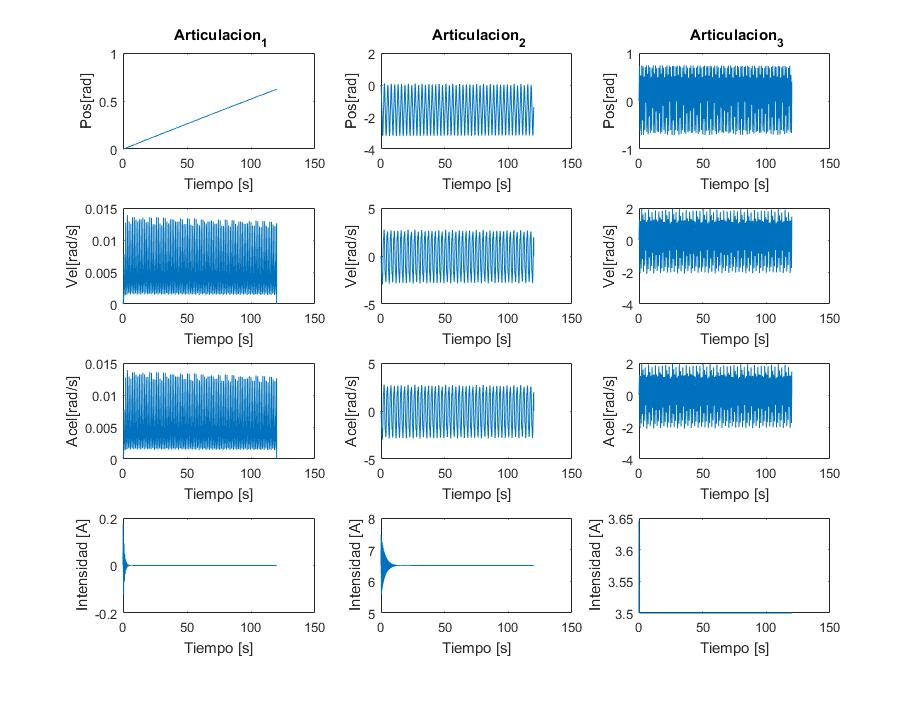
\includegraphics[width=0.3\textwidth]{graftheta10y11}
			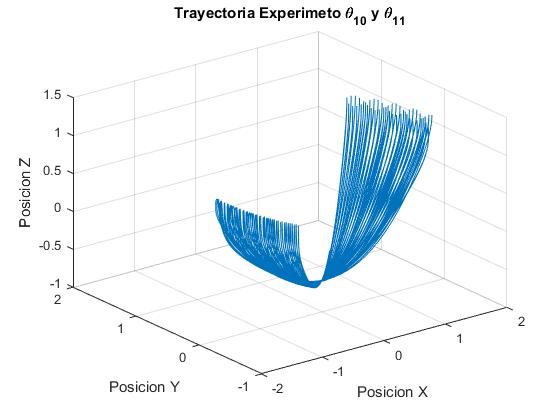
\includegraphics[width=0.3\textwidth]{Traytheta10y11}
			% \caption{Comparativa Variables articulares del modelo obtenido con medidas ideales y sin reductoras}
		\end{figure}
	
		\item Términos Viscosos $ \rightarrow $ valores de velocidad altas, y aceleraciones constantes
			\begin{figure}[h]
			\centering
			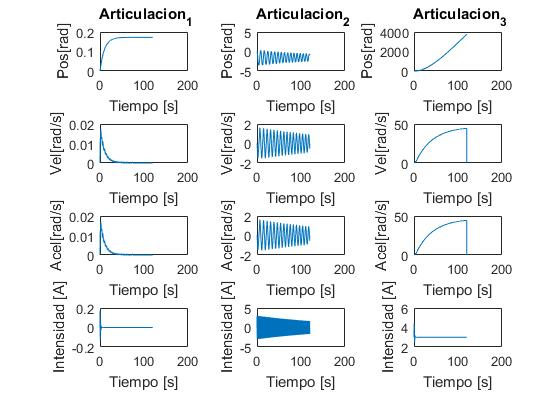
\includegraphics[width=0.3\textwidth]{graftheta9}
			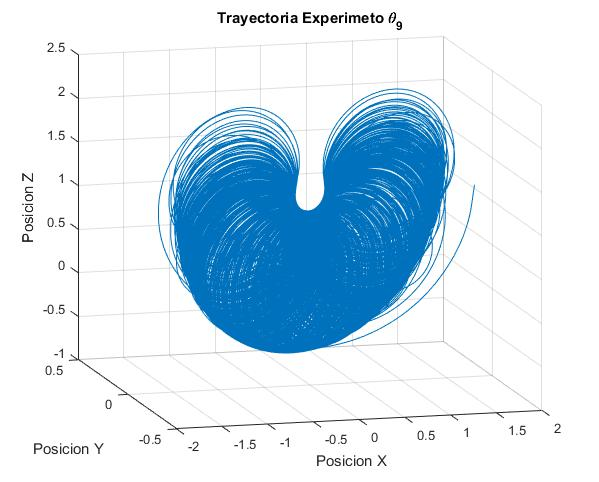
\includegraphics[width=0.3\textwidth]{Traytheta9}
			% \caption{Comparativa Variables articulares del modelo obtenido con medidas ideales y sin reductoras}
		\end{figure}

		\item Términos Inerciales $ \rightarrow $ consignas de aceleraciones altas; movimientos breves y bruscos en las articulaciones
		\begin{figure}[h]
			\centering
			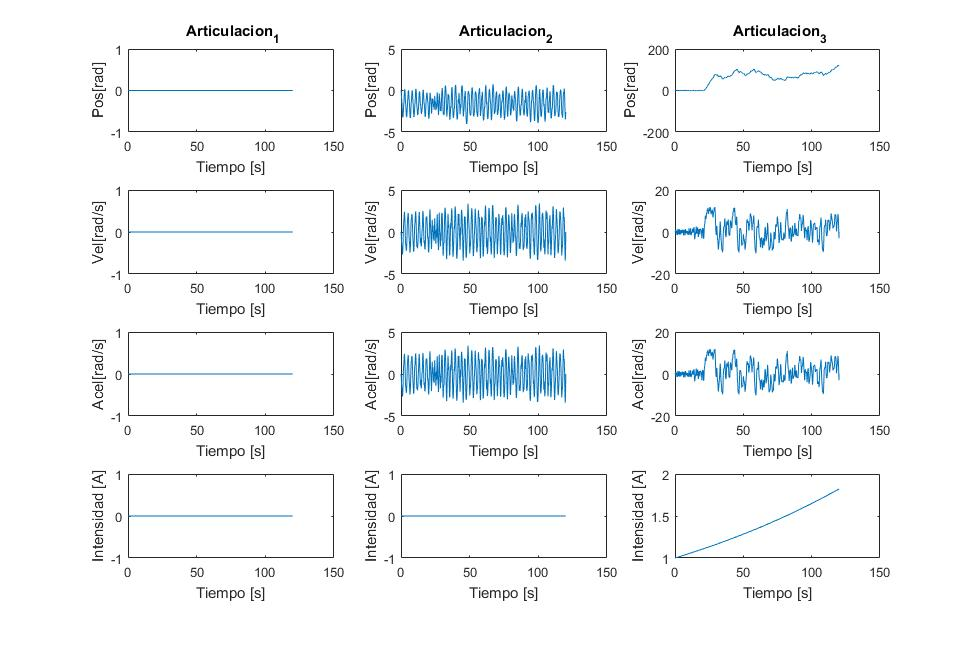
\includegraphics[width=0.3\textwidth]{graftheta8}
			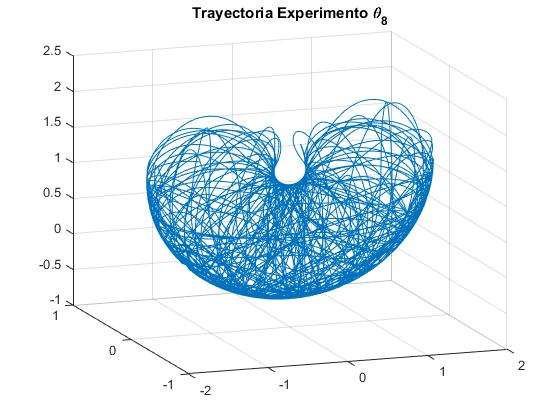
\includegraphics[width=0.3\textwidth]{Traytheta8}
			% \caption{Comparativa Variables articulares del modelo obtenido con medidas ideales y sin reductoras}
		\end{figure}
		

	\end{itemize}

	Para implementar las condiciones de funcionamiento han sido necesarias dos metodologias digerentes;
	por un lado, la propuesta en clase, que basa el diseño de las intensidades de entrada al robot,
	mediante dos señales senoidales, pudiendo variar de estas su amplitud, frecuencia y atenuacion; 
	y por otro, se ha usado señales exponenciales, en la que se han podido variar tanto la pendiente como la curvatura de la señal.	El uso de estas dos maneras de diseño de las señales de intensidad, es justificado debido a las problemáticas
	de los modelos a identificar.\\
	
	Se han identificado los modelos reales e ideales, con y sin reductoras, del robot propuesto. 
	En el caso del robot real, solo se han tomado los datos procedentes de las posiciones, a las que se le ha introducido,
	el efecto del encoder, para asemejar estos resultados a los obtenidos en la realidad; y sucesivas derivadas, para la obtención
	de las variables de velocidad y aceleración articulares; para ello, ha sido necesario introducir filtros Butterworth, que eliminen
	las componentes del ruido asociadas al efecto del encoder; es por ello, que ciertos experimentos, donde la variación
	de las posiciones, era fundamental para obtener las condiciones de funcionamiento mencionadas anteriormente, eran filtradas
	como ruido; es por esto, que se ha optado por señales exponenciales, para someter al robot real a condiciones de altas aceleraciones sin 
	necesidad de realizar una variación senoidal cuya frecuencia esté fuera de la banda de corte del filtrado.\\

	Aun así, las dificultades a la hora de la identificación de los parámetros dinámicos, se han dado principalmente,
	por el robot real sin reductoras; en este, se ha observado, que no solo se tiene que aumentar las intensidades
	de entrada de los experimentos, ya que, desde el el punto de la articulación, la ausencia de las reductoras se traduce en un par del motor menor;
	sino que, las perturbaciones externas que ocurren en las otras articulaciones o eslabones, cobran mucha mas relevancia, al no tener la amortiguación de las reductoras; lo que se traduce
	en un acoplamiento entre las propias barras del robot. Es decir, la ausencia de las reductoras, dificultan en gran medida,
	la búsqueda exclusiva del parámetro dinámico a identificar numéricamente.\\

	Finalmente, una vez definidas las consignas, para la identificación de los parámetros, las formas de ondas implementadas para ello,
	y los modelos sobre los que se han realizados dichos experimentos; se abordará la estadística detrás de la validación de estos experimentos, 
	dando como resultado la calidad de estos.\\
	Asumiendo que la metodologia expuesta en clase, sobre el calculo de la covarianza, en donde asumimos el error cometido como un ruido blanco,
	y que el algoritmo para calcular la desviación estándar relativa del parámetro, explicado en diapositivas, se ha implementado correctamente en la sintaxis de 
	Matlab, se exponen las condiciones de funcionamiento que aseguren la veracidad de este. Por un lado, y como se ha explicado en un inicio, el principio 
	seguido para la identificación, ha sido por caso redundante, lo que se ha asumido como, la toma de datos del orden de mil veces superior, al número de 
	parámetros dinámicos a identificar; por otro lado, no se puede tomar las medidas consecutivamente al tiempo de simulación, sino que se debe realizar una espera entre 
	la toma de los datos de salida del robot, evitando así los errores del sensorizado producidos por conservar propiedades de la medida una vez los estímulos iniciales han desaparecido, lo que viene
	a decir, evitar los errores por histéresis de los sensores, para ello se han tomado los datos cada 15-20 ud de tiempo de simulación, y para terminar de ha dado un umbral de error entorno al 5t.p.c. %Marco ponme esto bien pls q no se y me muero%
	de error sobre el valor real, que en el momento en el que se marque por debajo de este, se asumirá que el parámetro se ha obtenido correctamente.\\

	Algunas consideraciones finales, es necesario que a la hora de la realización del experimento, se tenga muy en cuenta que parámetros se están buscando, ya que,
	el algoritmo del cálculo de la covarianza, puede dar falsos positivos, en  parámetros que ni siquiera se están acentuando, es por ello, que es recomendable
	iniciar la identificación, por los modelos ideales, y posteriormente, con los datos del modelo real, teniendo al menos una base de apoyo a la hora de determinar que un parámetro es finalmente hallado.




	\subsection{Parámetros y modelos obtenidos}
	A continuación, se mostrarán los parámetros obtenidos para cada configuración del robot, así cómo la covarianza con la que se han obtenido los mismos.\\
	Para evitar repetir siempre los parámetros, se irán definiendo componente a componente, es decir, a continuación se definirá tetha con todos los parámetros y se dirá en cada caso concreto la posición del parámetro obtenido en el vector, el valor de dicho parámetro y la covarianza del mismo. \\

	Además de ello, se obtendrán las ecuaciones dinámicas que definen el comportamiento dinámico de las articulaciones del robot. Para obtener éstas ecuaciones, será necesario multiplicar la matriz $\gamma$ que posteriormente se definirá por la matriz $\theta$ con valores numericos. \\
	Una vez se tengan las ecuaciones dinámicas del robot, al igual que se hizo cuando se aplicó el algoritmo de \textit{Newton-Euler}, se irán derivando las expresiones respecto las posiciones, velocidades y aceleraciones articulares para obtener las matrices de inercias, matriz de terminos de Coirolis y la matriz formada por los términos gravitarios.\\

	Por último, cabe destacar que los modelos con medidas reales se han obtenido a partir de la posición del modelo real cuantizada, es decir, para obtener la velocidad y la aceleración fue necesario la aplicación de filtros no causales y la aplicación de filtros que limpien los ruidos.


La matriz $\gamma$ obtenida que, multiplicada por los valores numéricos de $\theta$, resultarán las ecuaciones dinámicas del robot estudiado, se muestra a continuación:



	\subsubsection{Robot medidas ideales con reductoras}
	Los parametros estimados, es decir, la matriz tetha linealmente independiente de 11 parámetros, obtenida para desarrollar el modelo del robot con medidas ideales con reductoras en los motores será:
	\begin{center}
		\begin{tabular}{| c | c | c |}

			\hline
			Parametro estimado & Valor obtenido & Covarianza obtenida \\
			\hline
			$\theta(1) $ & 15.6322 & 0.0338 \\
			\hline
			$\theta(2) $ & 0.0012 & 0.0218 \\
			\hline
			$\theta(3) $ & 7.389 & 0.0481 \\
			\hline
			$\theta(4) $ & 55.1139 & 0.00081 \\
			\hline
			$\theta(5) $ & 0.00085 & 0.02744 \\
			\hline
			$\theta(6) $ & 2.0841 & 0.047868 \\
			\hline
			$\theta(7) $ & -2.0414 & 0.00623 \\
			\hline
			$\theta(8) $ & 0.051 & 0.00113 \\
			\hline
			$\theta(9) $ & 0.0015 & 0.033 \\
			\hline
			$\theta(10) $ & -6.665 & 0.00054 \\
			\hline
			$\theta(11) $ & -2.222 & 0.00113 \\
			\hline


		\end{tabular}
	\end{center}
Por lo tanto, tras multiplicar $\gamma$ y $\theta$ y derivar respecto a las variables articulares, se definirán las ecuaciones dinámicas del robot ideal con reductoras cómo:\\
\[
	\begin{pmatrix}
	Kt_{1}R_{1}Im_{1} \\
	Kt_{2}R_{2}Im_{2} \\
	Kt_{3}R_{3}Im_{3}
	\end{pmatrix} =
	\begin{pmatrix}
	Ma_{1,1} & 0 & 0 \\
	0 & Ma_{2,2} & Ma_{2,3}\\
	0 & Ma_{3,2} & 2.463
	\end{pmatrix}
	\begin{pmatrix}
	\ddot{q_{1}} \\
	\ddot{q_{2}}  \\
	\ddot{q_{3}}
\end{pmatrix} +
\begin{pmatrix}
	Va_{1,1}\\
	Va_{2,1} \\
  Va_{3,1}
\end{pmatrix}
\begin{pmatrix}
		\dot{q_{1}} \\
		\dot{q_{2}}  \\
		\dot{q_{3}}
\end{pmatrix} +
\begin{pmatrix}
 	0 \\
  1.81cos(q_{2} + q_{3}) + 5.44cos(q_{2}) \\
                 4.15cos(q_{2} + q_{3})
\end{pmatrix}
\]

\begin{itemize}
	\item $ Ma_{1,1}=0.0889cos(2q_{2} + q_{3}) + 0.119cos(2q_{2}) + 0.0889cos(q_{3}) + 0.0294cos(2q_{2} + 2q_{3}) + 1.15$ \\ \vspace{0.2cm}
	\item $ Ma_{2,2}=0.3703cos(q_{3}) + 5.83$ \\ \vspace{0.2cm}
	\item $ Ma_{2,3}=0.1851cos(q_{3}) + 0.126  $ \\ \vspace{0.2cm}
	\item $ Ma_{3,2}=0.4232cos(q_{3}) + 0.288  $ \\ \vspace{0.2cm}
	\item $ Va_{1,1}=0.178\dot{q_1}\dot{q_2}sin(2q_2 + q_3) + 0.0887\dot{q_1}\dot{q_3}sin(2q_2 + q_3) + 0.235\dot{q_1}\dot{q_2}sin(2q2) + 0.0887\dot{q_3}\dot{q_1}sin(q_3) + $ \\ \vspace{0.1cm}
	 $+0.059\dot{q_1}\dot{q_2}sin(2q_2 + 2q_3) + 0.059\dot{q_1}\dot{q_3}sin(2q_2 + 2q_3) - 0.12\dot{q_1} $ \\ \vspace{0.2cm}
	 \item $ Va_{2,1}=0.0638\dot{q_2} - 0.185\dot{q_3}^{2}sin(q_3) + 0.0613\dot{q_1}^{2}sin(2q_2 + 2q_3) + 0.185\dot{q_1}^{2}sin(2q_2 + q_3) + 0.248\dot{q_1}^{2}sin(2q_2) - $ \\ \vspace{0.1cm}
	 $ -0.37\dot{q_2}\dot{q_3}sin(q_3) $\\ \vspace{0.2cm}
	 \item $ Va_{3,1}= 0.0643\dot{q_3} + 0.212\dot{q_1}^{2}sin(q3) + 0.423\dot{q_2}^{2}sin(q_3) + 0.14\dot{q_1}^{2}sin(2q_2 + 2q_3) + 0.212\dot{q_1}^{2}sin(2q_2 + q_3) $
\end{itemize}

\newpage
\subsubsection{Robot medidas ideales sin reductoras}
Los parametros estimados, es decir, la matriz tetha linealmente independiente de 11 parámetros, obtenida para desarrollar el modelo del robot con medidas ideales sin reductoras en los motores será:
\begin{center}
	\begin{tabular}{| c | c | c |}

		\hline
		Parametro estimado & Valor obtenido & Covarianza obtenida \\
		\hline
		$\theta(1) $ & -9.31476 & 0.00364 \\
		\hline
		$\theta(2) $ & 0.001193 & 2.868 \\
		\hline
		$\theta(3) $ & 7.3803 & 0.00036 \\
		\hline
		$\theta(4) $ & -7.2341 & 0.00369 \\
		\hline
		$\theta(5) $ & 0.00121 & 5.890 \\
		\hline
		$\theta(6) $ & 2.078 & 0.00358 \\
		\hline
		$\theta(7) $ & -2.0335 & 0.00359 \\
		\hline
		$\theta(8) $ & 0.051 & 0.0148 \\
		\hline
		$\theta(9) $ & 0.00146 & 2.19 \\
		\hline
		$\theta(10) $ & -6.6585 & 0.003621 \\
		\hline
		$\theta(11) $ & -2.222 & 0.00356 \\
		\hline
	\end{tabular}
\end{center}
Por lo tanto, tras multiplicar $\gamma$ y $\theta$ y derivar respecto a las variables articulares, se definirán las ecuaciones dinámicas del robot ideal con reductoras cómo:\\
\[
	\begin{pmatrix}
	Kt_{1}R_{1}Im_{1} \\
	Kt_{2}R_{2}Im_{2} \\
	Kt_{3}R_{3}Im_{3}
	\end{pmatrix} =
	\begin{pmatrix}
	Ma_{1,1} & 0 & 0 \\
	0 & Ma_{2,2} & Ma_{2,3}\\
	0 & Ma_{3,2} & 4.47
	\end{pmatrix}
	\begin{pmatrix}
	\ddot{q_{1}} \\
	\ddot{q_{2}}  \\
	\ddot{q_{3}}
\end{pmatrix} +
\begin{pmatrix}
	Va_{1,1}\\
	Va_{2,1} \\
  Va_{3,1}
\end{pmatrix}
\begin{pmatrix}
		\dot{q_{1}} \\
		\dot{q_{2}}  \\
		\dot{q_{3}}
\end{pmatrix} +
\begin{pmatrix}
	0 \\
54.3cos(q_{2} + q_{3}) + 163cos(q_{2}) \\
62.1cos(q_{2} + q_{3})
\end{pmatrix}
\]

\begin{itemize}
	\item $ Ma_{1,1}=4.434cos(2q_{2} + q_{3}) + 5.937cos(2q_{2}) + 4.434cos(q_{3}) + 1.469cos(2q_{2} + 2q_{3}) + 7.693$ \\ \vspace{0.2cm}
	\item $ Ma_{2,2}=11.08cos(q_{3}) + 18.99$ \\ \vspace{0.2cm}
	\item $ Ma_{2,3}=5.542cos(q_{3}) + 3.784$ \\ \vspace{0.2cm}
	\item $ Ma_{3,2}=6.334cos(q3) + 4.325$ \\ \vspace{0.2cm}
	\item $ Va_{1,1}=-8.84\dot{q_1}\dot{q_2}sin(2q_2 + q_3) - 4.429\dot{q_1}\dot{q_3}sin(2q_2 + q_3)  -11.85\dot{q_1}\dot{q_2}sin(2q_2) - 4.429\dot{q_1}\dot{q_3}sin(q_3)-$ \\ \vspace{0.1cm}
	 $-2.924\dot{q_1}\dot{q_2}sin(2q_2 + 2q_3) - 2.924\dot{q_1}\dot{q_3}sin(2q_2 + 2q_3) 0.002387\dot{q_1} $ \\ \vspace{0.2cm}
	 \item $ Va_{2,1}=0.00304\dot{q_2} - 5.54\dot{q_3}^{2}sin(q_{3}) + 1.84\dot{q_{1}}^{2}sin(2q_{2} + 2q_{3}) + 5.54\dot{q_1}^{2}sin(2q_{2} + q_{3}) + $ \\ \vspace{0.1cm}
	 $ + 7.42\dot{q_1}^{2}sin(2q_{2}) - 11.1\dot{q_{2}}\dot{q_{3}}sin(q_{3}) ) $\\ \vspace{0.2cm}
	 \item $ Va_{3,1}=0.00418\dot{q_3} + 3.17\dot{q_1}^{2}sin(q_{3}) + 6.33\dot{q_2}^{2}sin(q_{3}) + 2.1\dot{q_1}^{2}sin(2q_{2} + 2q_{3}) + 3.17\dot{q_1}^{2}sin(2q_{2} + q_{3}) $
\end{itemize}
\newpage
\subsubsection{Robot medidas reales con reductoras}
Los parametros estimados, es decir, la matriz tetha linealmente independiente de 11 parámetros, obtenida para desarrollar el modelo del robot con medidas reales con reductoras en los motores será:
\begin{center}
	\begin{tabular}{| c | c | c |}

		\hline
		Parametro estimado & Valor obtenido & Covarianza obtenida \\
		\hline
		$\theta(1) $ & 16.995 & 4.0573 \\
		\hline
		$\theta(2) $ & 0.00122 & 0.2538 \\
		\hline
		$\theta(3) $ & 12.393 & 1.291 \\
		\hline
		$\theta(4) $ & 38.28 & 1.9472 \\
		\hline
		$\theta(5) $ & 0.00129 & 0.941 \\
		\hline
		$\theta(6) $ & 1.434 & 0.917 \\
		\hline
		$\theta(7) $ & 4.0372 & 4.545 \\
		\hline
		$\theta(8) $ & 0.0491 & 1.234 \\
		\hline
		$\theta(9) $ & 0.00151 & 1.468 \\
		\hline
		$\theta(10) $ & -6.6722 & 0.003858 \\
		\hline
		$\theta(11) $ & -2.199 & 0.008916 \\
		\hline
	\end{tabular}
\end{center}
Por lo tanto, tras multiplicar $\gamma$ y $\theta$ y derivar respecto a las variables articulares, se definirán las ecuaciones dinámicas del robot ideal con reductoras cómo:\\

\[
	\begin{pmatrix}
	Kt_{1}R_{1}Im_{1} \\
	Kt_{2}R_{2}Im_{2} \\
	Kt_{3}R_{3}Im_{3}
	\end{pmatrix} =
	\begin{pmatrix}
	Ma_{1,1} & 0 & 0 \\
	0 & Ma_{2,2} & Ma_{2,3}\\
	0 & Ma_{3,2} & 2.78
	\end{pmatrix}
	\begin{pmatrix}
	\ddot{q_{1}} \\
	\ddot{q_{2}}  \\
	\ddot{q_{3}}
\end{pmatrix} +
\begin{pmatrix}
	Va_{1,1}\\
	Va_{2,1} \\
  Va_{3,1}
\end{pmatrix}
\begin{pmatrix}
		\dot{q_{1}} \\
		\dot{q_{2}}  \\
		\dot{q_{3}}
\end{pmatrix} +
\begin{pmatrix}
	0																	\\
1.796cos(q_2 + q_3) + 5.449cos(q_2) \\
4.105cos(q_2 + q_3)
\end{pmatrix}
\]

\begin{itemize}
	\item $ Ma_{1,1}=0.088cos(2q_2 + q_3) + 0.019cos(2q_2) + 0.088cos(q_3) + 0.0417cos(2q_{2} + 2q_{3}) + 1.29$ \\ \vspace{0.2cm}
	\item $ Ma_{2,2}= 0.366cos(q_3) + 4.6$ \\ \vspace{0.2cm}
	\item $ Ma_{2,3}=0.183cos(q_3) + 0.293$ \\ \vspace{0.2cm}
	\item $ Ma_{3,2}=  0.419cos(q_3) + 0.67$ \\ \vspace{0.2cm}
	\item $ Va_{1,1}=-0.1758\dot{q_1}\dot{q_2}sin(2q_2 + q_3) - 0.08791\dot{q_1}\dot{q_3}sin(2q_2 + q_3) - 0.03796\dot{q_1}\dot{q_2}sin(2q_2) -$ \\ \vspace{0.1cm}
	 $ - 0.08791\dot{q_1}\dot{q_3}sin(q_3) - 0.08325\dot{q_1}\dot{q_2}sin(2q_2 + 2q_3) - 0.08325\dot{q_1}\dot{q_3}sin(2q_2 + 2q_3) + 0.1223\dot{q_1)}$ \\ \vspace{0.2cm}
	 \item $ Va_{2,1}=0.0969\dot{q_2} - 0.183\dot{q_3}^{2}sin(q_3) + 0.0868\dot{q_1}^{2}sin(2q_{2} + 2q_{3}) + 0.183\dot{q_1}^{2}sin(2q_2 + q_3) + $ \\ \vspace{0.1cm}
	 $ + 0.0396\dot{q_1}^{2}sin(2q_{2}) - 0.366\dot{q_2}\dot{q_3}sin(q_3) $\\ \vspace{0.2cm}
	 \item $ Va_{3,1}=0.0648\dot{q_3} + 0.209\dot{q_1}^{2}sin(q_3) + 0.419\dot{q_2}^{2}sin(q_3) + 0.199\dot{q_1}^{2}sin(2q_2 + 2q_3) + 0.209\dot{q_1}^{2}sin(2q_2 + q_3) $
\end{itemize}

\newpage
\subsubsection{Robot medidas reales sin reductoras}
Los parametros estimados, es decir, la matriz tetha linealmente independiente de 11 parámetros, obtenida para desarrollar el modelo del robot con medidas reales sin reductoras en los motores será:
\begin{center}
	\begin{tabular}{| c | c | c |}

		\hline
		Parametro estimado & Valor obtenido & Covarianza obtenida \\
		\hline
		$\theta(1) $ & - & - \\
		\hline
		$\theta(2) $ & - & - \\
		\hline
		$\theta(3) $ & - & - \\
		\hline
		$\theta(4) $ & - & - \\
		\hline
		$\theta(5) $ & - & - \\
		\hline
		$\theta(6) $ & - & - \\
		\hline
		$\theta(7) $ & - & - \\
		\hline
		$\theta(8) $ & - & - \\
		\hline
		$\theta(9) $ & - & - \\
		\hline
		$\theta(10) $ & - & - \\
		\hline
		$\theta(11) $ & - & - \\
		\hline
	\end{tabular}
\end{center}
Por lo tanto, tras multiplicar $\gamma$ y $\theta$ y derivar respecto a las variables articulares, se definirán las ecuaciones dinámicas del robot ideal con reductoras cómo:\\
\[
	\begin{pmatrix}
	Kt_{1}R_{1}Im_{1} \\
	Kt_{2}R_{2}Im_{2} \\
	Kt_{3}R_{3}Im_{3}
	\end{pmatrix} =
	\begin{pmatrix}
	Ma_{1,1} & 0 & 0 \\
	0 & Ma_{2,2} & Ma_{2,3}\\
	0 & Ma_{3,2} & -
	\end{pmatrix}
	\begin{pmatrix}
	\ddot{q_{1}} \\
	\ddot{q_{2}}  \\
	\ddot{q_{3}}
\end{pmatrix} +
\begin{pmatrix}
	Va_{1,1}\\
	Va_{2,1} \\
  Va_{3,1}
\end{pmatrix}
\begin{pmatrix}
		\dot{q_{1}} \\
		\dot{q_{2}}  \\
		\dot{q_{3}}
\end{pmatrix} +
\begin{pmatrix}
-	\\
- \\
-
\end{pmatrix}
\]

\begin{itemize}
	\item $ Ma_{1,1}=$ \\ \vspace{0.2cm}
	\item $ Ma_{2,2}= $ \\ \vspace{0.2cm}
	\item $ Ma_{2,3}=$ \\ \vspace{0.2cm}
	\item $ Ma_{3,2}=  $ \\ \vspace{0.2cm}
	\item $ Va_{1,1}= $ \\ \vspace{0.2cm}
	 \item $ Va_{2,1}= $ \\ \vspace{0.2cm}
	 \item $ Va_{3,1}= $
\end{itemize}


\newpage
\subsection{Verificación de los modelos obtenidos}
Tras obtener éstos modelos, se hará una simple prueba antes de comenzar a controlar el robot para poder analizar la bondad del modelo obtenido.\\
Se ha optado por, para comprobar dicha bondad, introducirle al robot dado por el profesor, es decir, el robot real valores de intensidades unitarios y lo
mismo al modelo, de ese modo se podrá observar y comparar la respuesta del robot real y el modelo obtenido.\\

Cabe destacar que, debido a que no se controlará el robot durante más de 5 segudos aproximadamente, durante ese tiempo es dónde interesa observar la bondad del modelo.
\subsubsection{Robot medidas ideales con reductoras}
En primer lugar, se mostrará cómo responden las variables articulares del modelo obtenido frente a las del robot real. La gráfica que se muestra es la obtenida empleando las medidas ideales de éstas variables articulares tanto del robot real cómo del modelo:

\begin{figure}[h!]
	\centering
	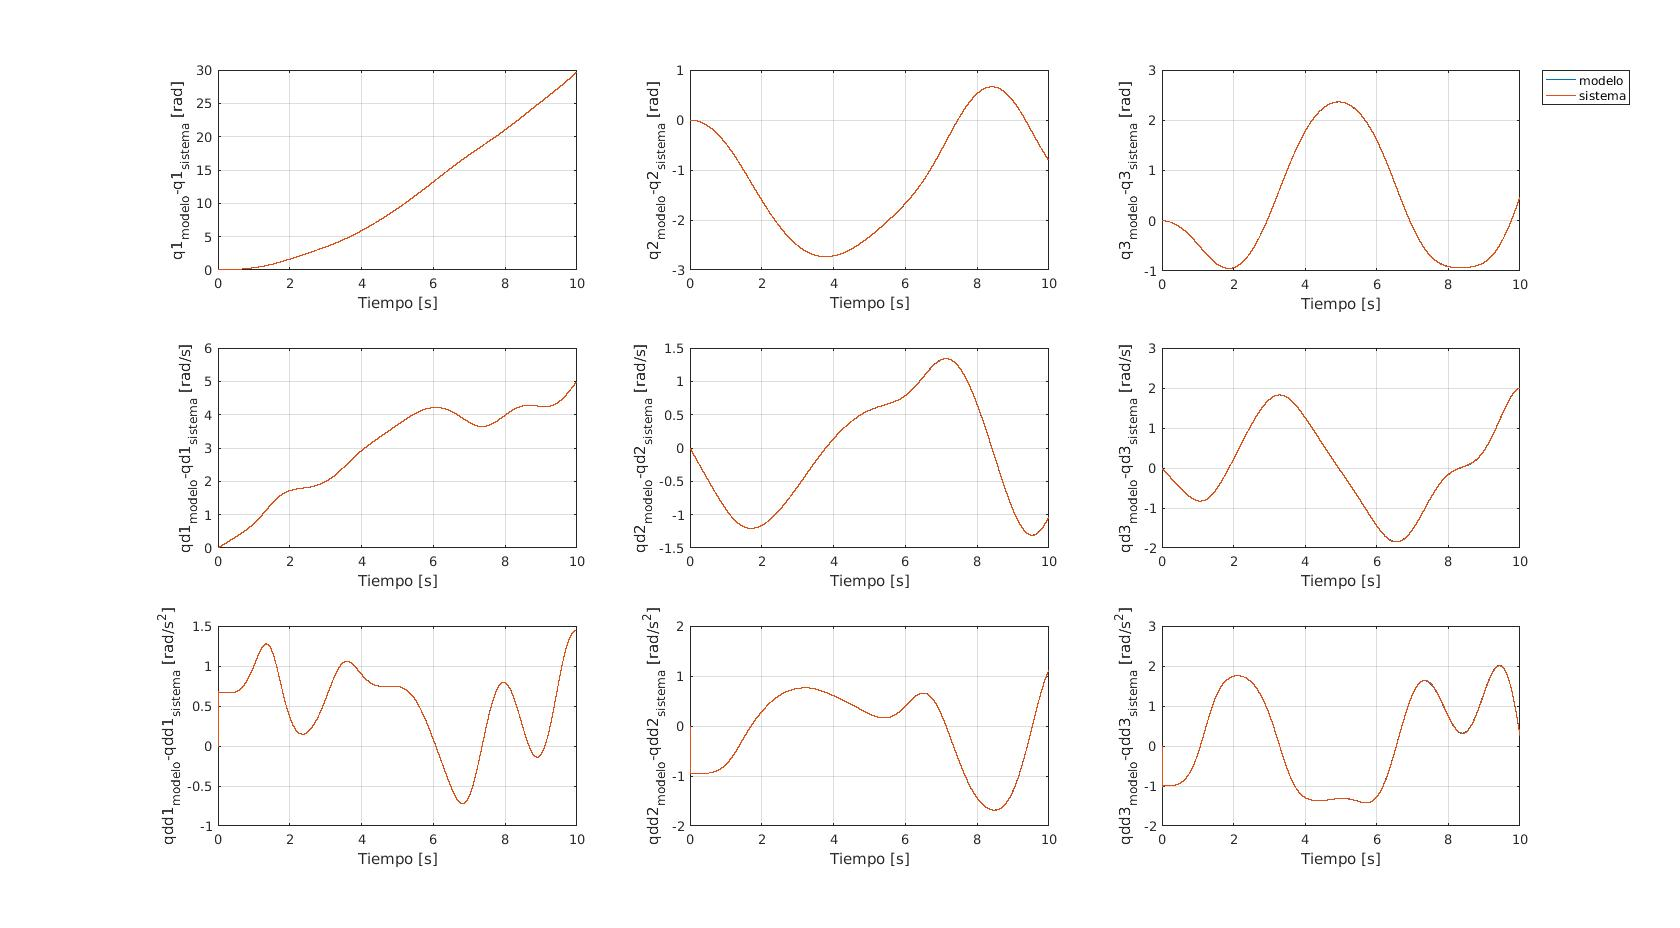
\includegraphics[width=1\textwidth]{EstimacParam_SisMod_In1_IdealCR}
	\caption{Comparativa Variables articulares del modelo obtenido con medidas ideales y reductoras}
\end{figure}

Cómo se puede observar, la magnitud del error será muy baja, por tanto, eso conllevará que se han estimado los parámetros dinámicos del robot con un bajo error entre los parámetros reales.\\
\newpage
A continuación, se mostrará la gráfica del error en las variables articulares:

\begin{figure}[h!]
	\centering
	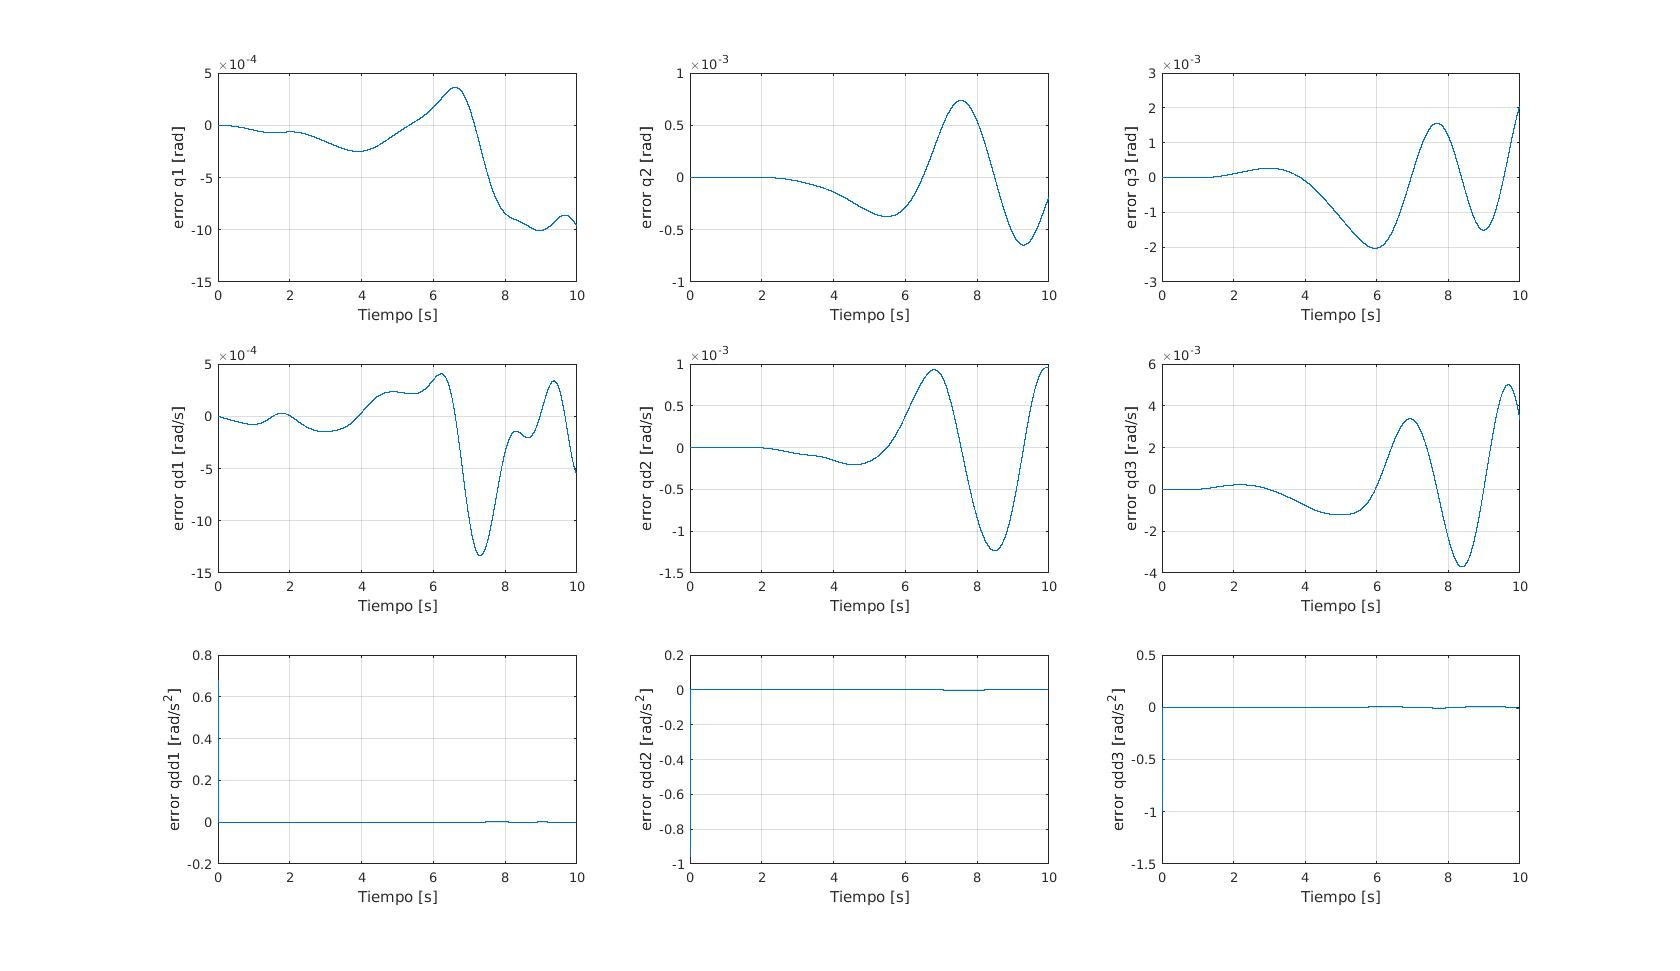
\includegraphics[width=1\textwidth]{EstimacParam_SisModError_In1_IdealCR}
	\caption{Error del modelo obtenido con medidas ideales y reductoras}
\end{figure}

\subsubsection{Robot medidas ideales sin reductoras}
En éste caso, se realizará la misma comparativa que en el caso anterior, con la salvedad es que en el modelo obtenido ahora, se suponen que no se tienen reductoras.\\
Cabe destacar que nos interesa el modelo del robot a bjos tiempos, es decir, los primeros 5 segundos de la simulación, pues no se va a querer controlar el robot en trayectorias que duren más tiempo. Se ha graficado más tiempo para que se observe que, cuando empieza a pasar más del tiempo que se desea controlar, los errores comienzan a incrementarse.\\
A continuación, se mostrará la gráfica resultando al excitar el modelo del sistema y el robot real con intensidades constantes y unitarias.

\newpage
\begin{figure}[h!]
	\centering
	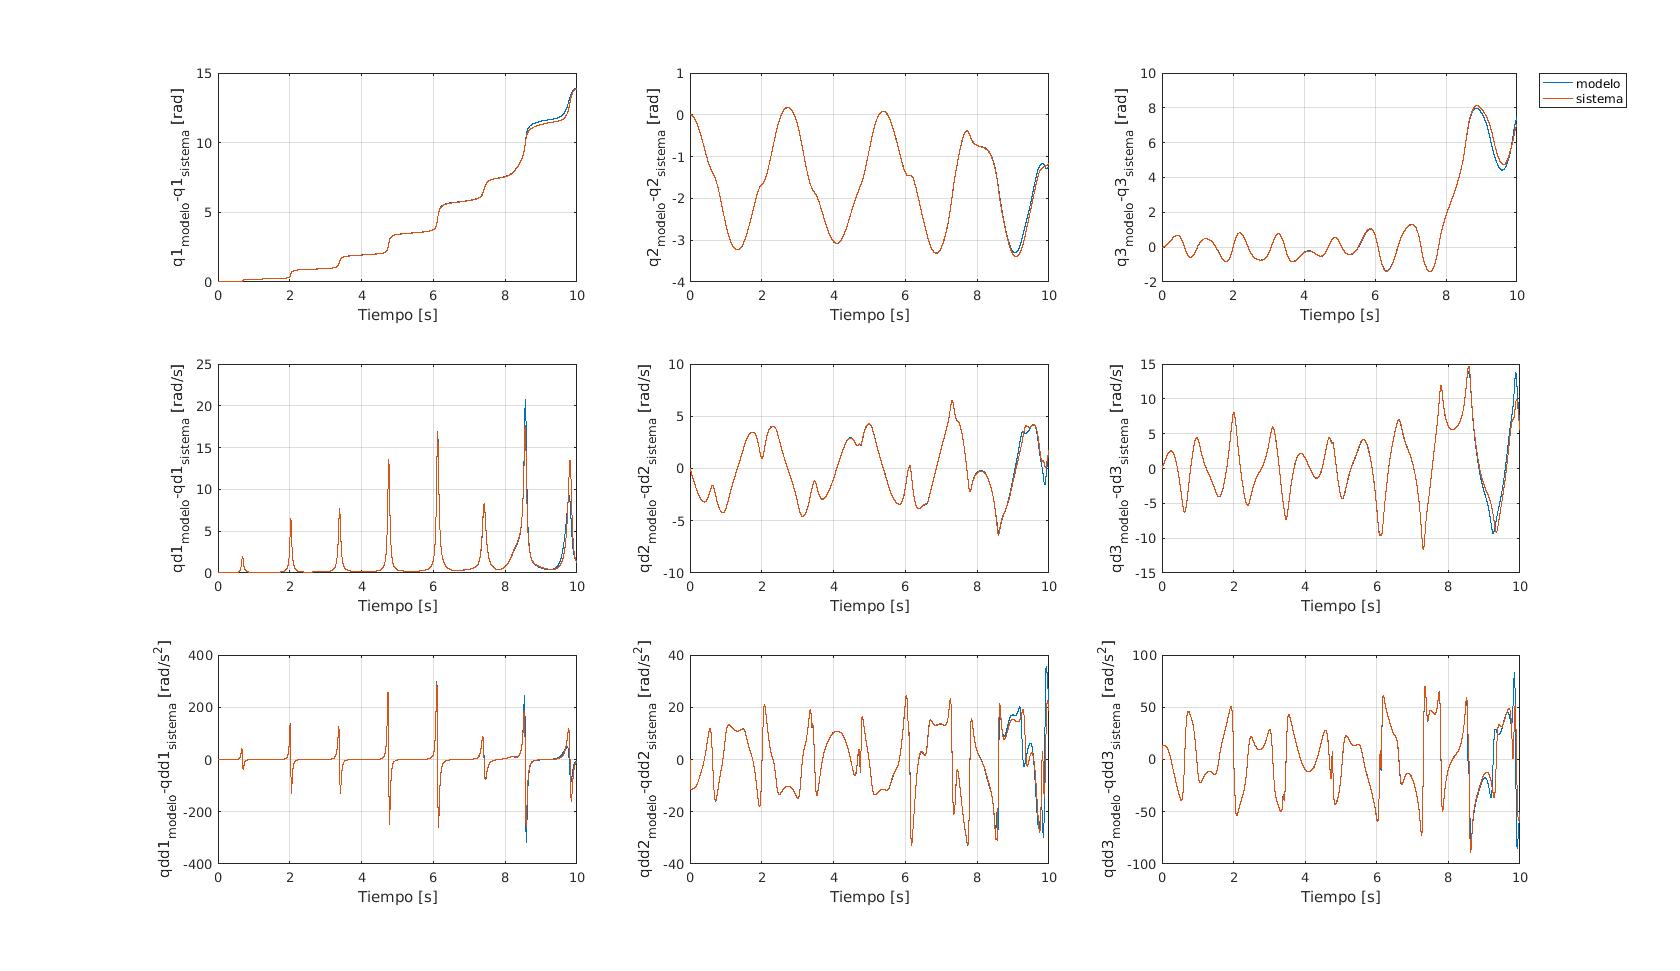
\includegraphics[width=1\textwidth]{EstimacParam_SisMod_In1_IdealSR}
	\caption{Comparativa Variables articulares del modelo obtenido con medidas ideales y sin reductoras}
\end{figure}

Cómo se puede observar, al igual que antes, cuándo se emplean medidas ideales para estimar los parámetros dinámicos del robot y obtener un modelo del mismo, se obtendrán buenos modelos, debido a que cómo se indico antes, las medidas son ideales. \\
Por tanto, a continuación se mostrará la gráfica de los errores de las variables articulares:

\begin{figure}[h!]
	\centering
	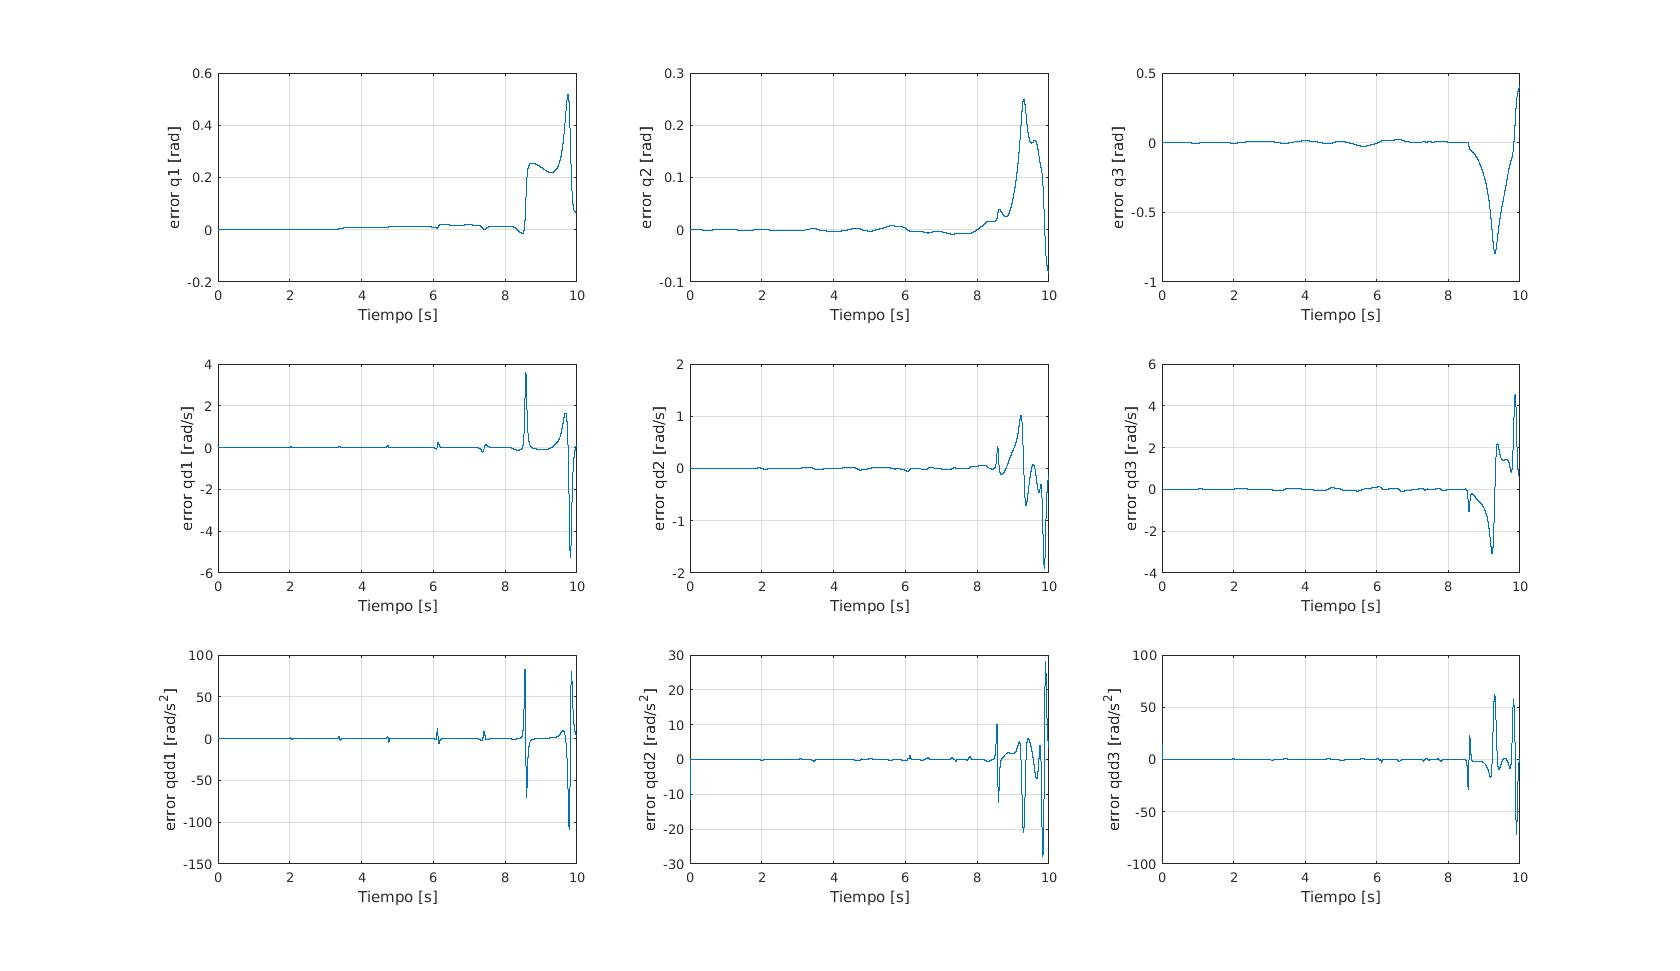
\includegraphics[width=1\textwidth]{EstimacParam_SisModError_In1_IdealSR}
	\caption{Error del modelo obtenido con medidas ideales y sin reductoras}
\end{figure}

\subsubsection{Robot medidas reales con reductoras}
Aunque se haya obtenido el modelo con medidas reales suponiendo que no se tienen tacómetros y que, por tanto, no se puede conocer la velocidad articular del robot, para realizar análisis de control y para análizar el modelo obtenido sí se conocerá la velocidad articular, es decir, se supondrá que se tienen tacómetros. De ese modo se evitará la necesidad de implementar un filtro no causal. \\
Los filtros no causales se caracterizan por el hecho de se emplean valores futuros de la señal, algo que sólo se podrá hacer de manera computacional una vez se hayan tomado todos los datos.\\

Por tanto, se compararán las medidas reales de velocidad y posición del robot con las medidas ideales del modelo obtenido. La grafica comparativa se muestra a continuación:

\begin{figure}[h!]
	\centering
	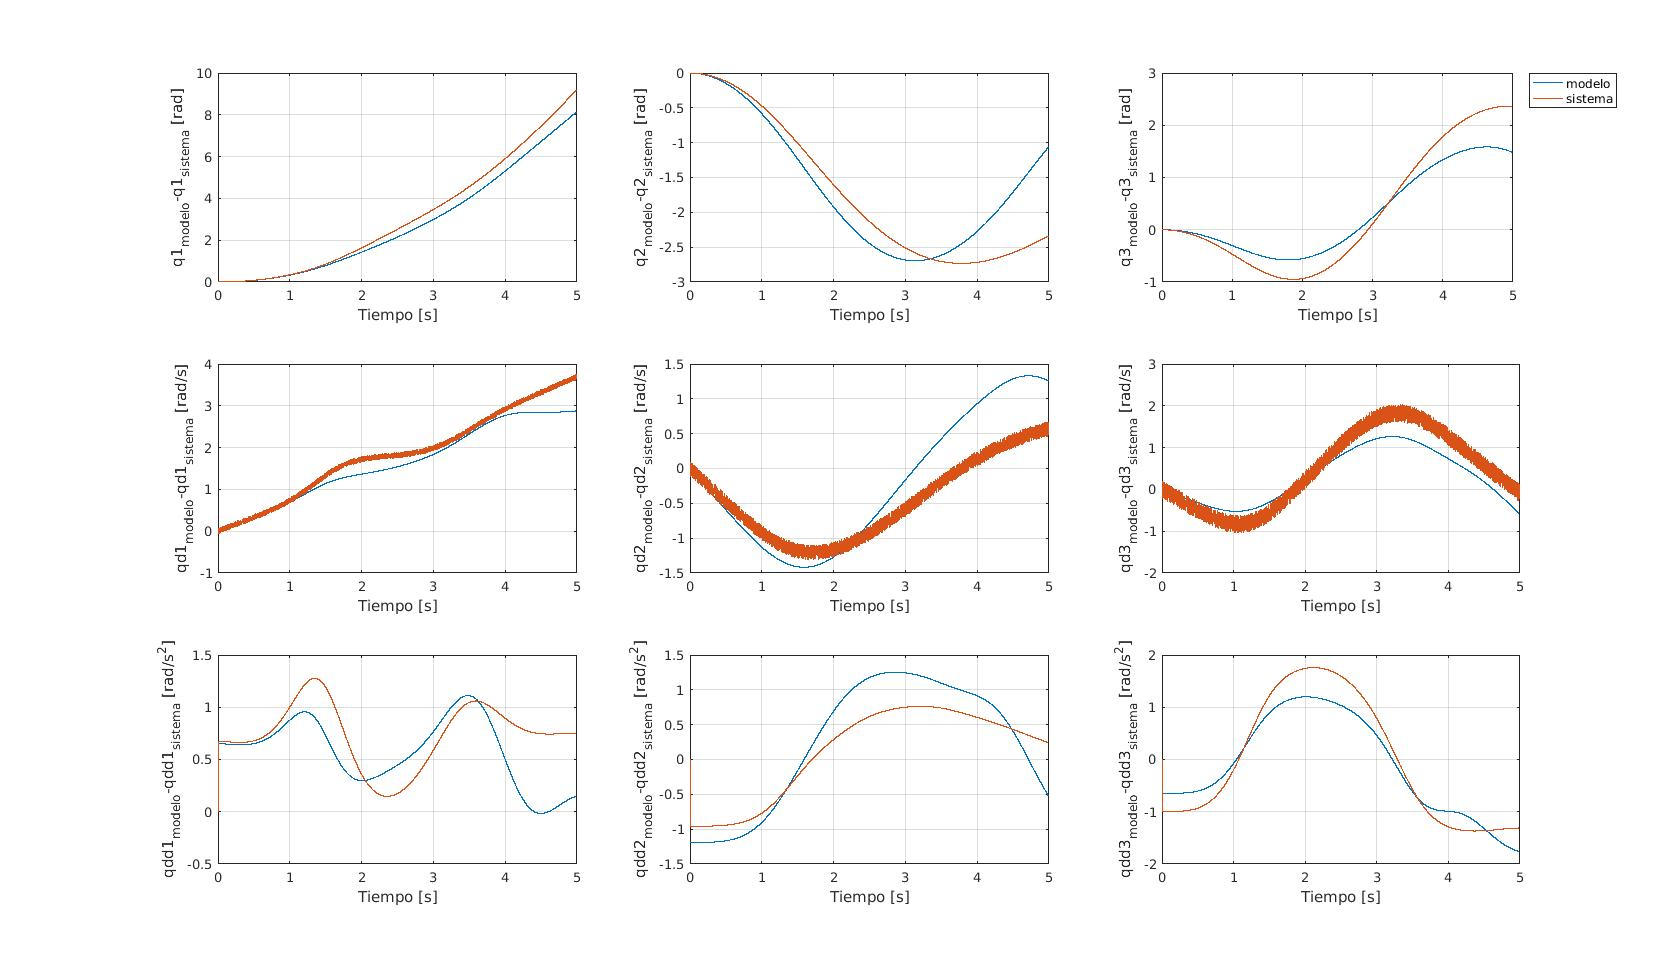
\includegraphics[width=1\textwidth]{EstimacParam_SisMod_In1_RealCR}
	\caption{Comparativa Variables articulares del modelo obtenido con medidas reales y reductoras}
\end{figure}

En éste caso, se observa cómo al emplear medidas reales para obtener el modelo dinámico del robot y al haber tenido que emplear filtros computacionales para conocer velocidades y aceleraciones del robot, el modelo obtenido no será tan bueno cómo en el caso en el que se usaron medidas ideales. Sin embargo, debido a que no posee un elevado orden de magnitud, se asumirá dicho error y se tomará el modelo cómo válido.\\
Ademas de ello, se observa que aparece cierto desfase entre el modelo obtenido y el robot real, éste desfase es debido a la aplicación de filtros a la señal. Cuando se emplean filtros hay que tener en cuenta que éstos introducen un cierto desfase, por tanto, será necesario encontrar un compomiso entre cuán bueno se quiere que sea el filtro y cuánto desfase se está dispuesto a asumir. En éste caso, debido a que nos encontramos en un proyecto basado en la simulación, se aceptará un cierto desfase a cambio de haber diseñado buenos filtros para las señales.

\newpage
Por tanto, la magnitud de los errores obtenidos se muestra a continuación:

\begin{figure}[h!]
	\centering
	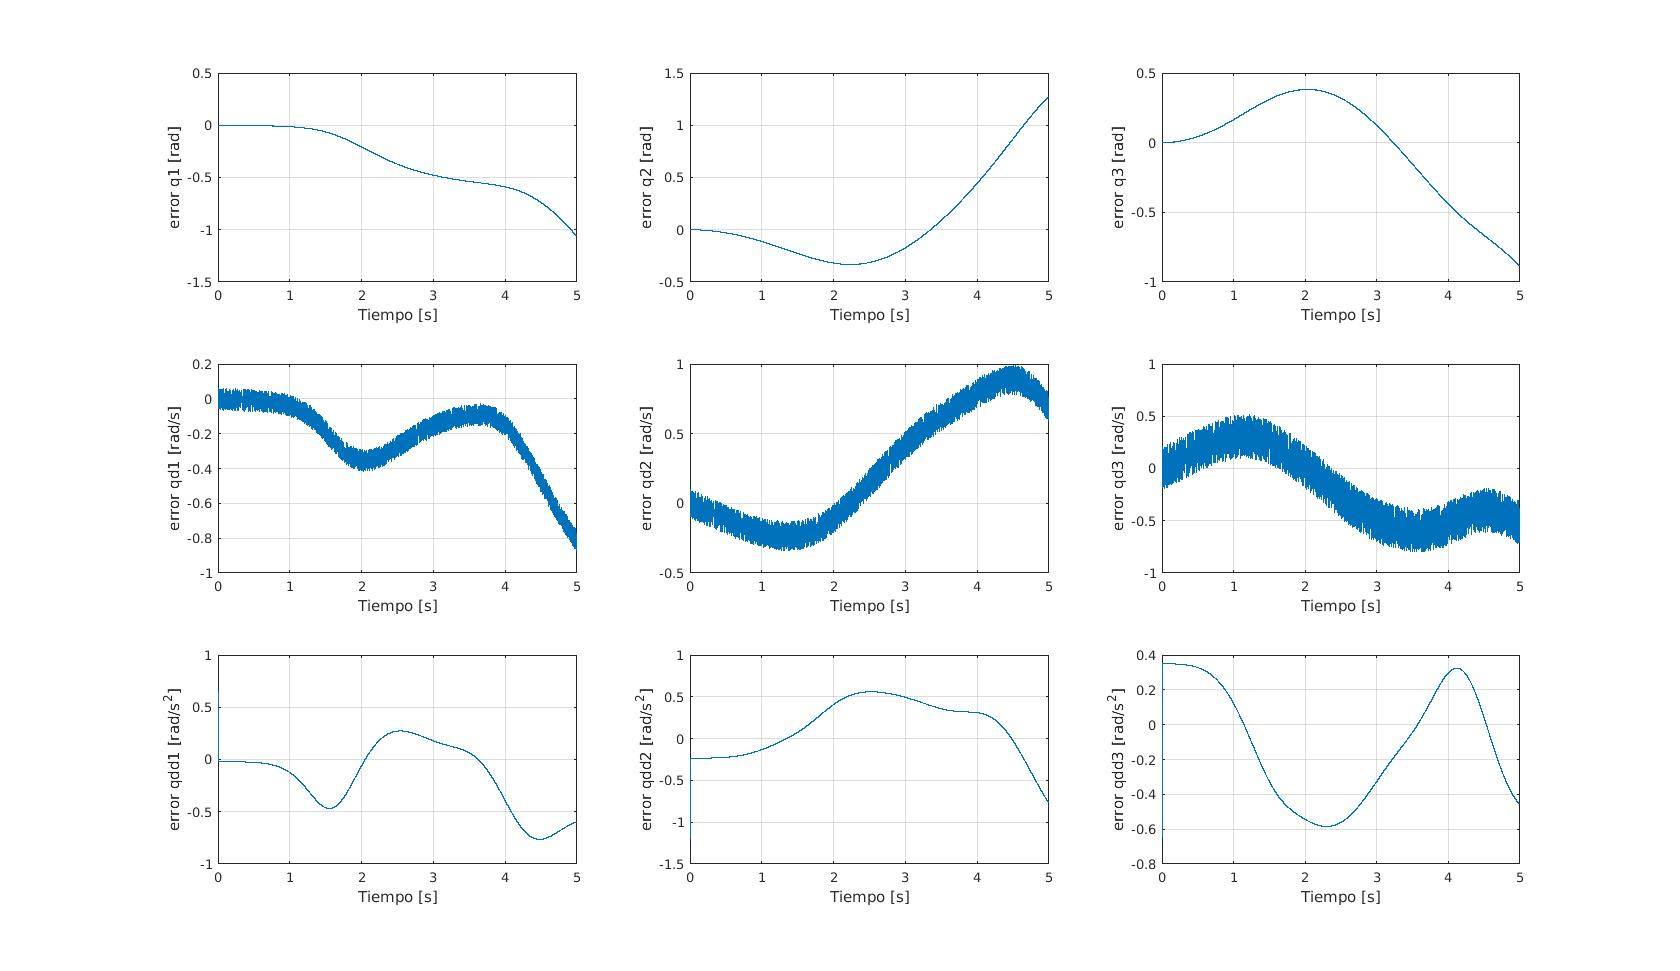
\includegraphics[width=1\textwidth]{EstimacParam_SisModError_In1_RealCR}
	\caption{Error del modelo obtenido con medidas reales y reductoras}
\end{figure}

\subsubsection{Robot medidas reales sin reductoras}
